\documentclass[landscape]{proc}
\usepackage{amscd,amsmath,amsthm,amssymb}
\usepackage{enumerate,varioref}
\usepackage{epsfig}
\usepackage{graphicx}
\usepackage{mathtools}
\usepackage{tikz}
\newtheorem{thm}{Theorem}
\newtheorem{cor}[thm]{Corollary}
\newtheorem{lem}[thm]{Lemma}
\newtheorem{prop}[thm]{Proposition}
\theoremstyle{definition}
\newtheorem{defn}[thm]{Definition}
\theoremstyle{remark}
\newtheorem{ex}[thm]{Example}
\newtheorem{rem}[thm]{Remark}
\numberwithin{equation}{subsection}
\newcommand{\R}{\mathbb{R}}
\newcommand{\Z}{\mathbb{Z}}
\newcommand{\C}{\mathbb{C}}
\newcommand{\Q}{\mathbb{Q}}
\newcommand{\lh}{\lim_{h\rightarrow 0}}
\begin{document}
	
	
\[
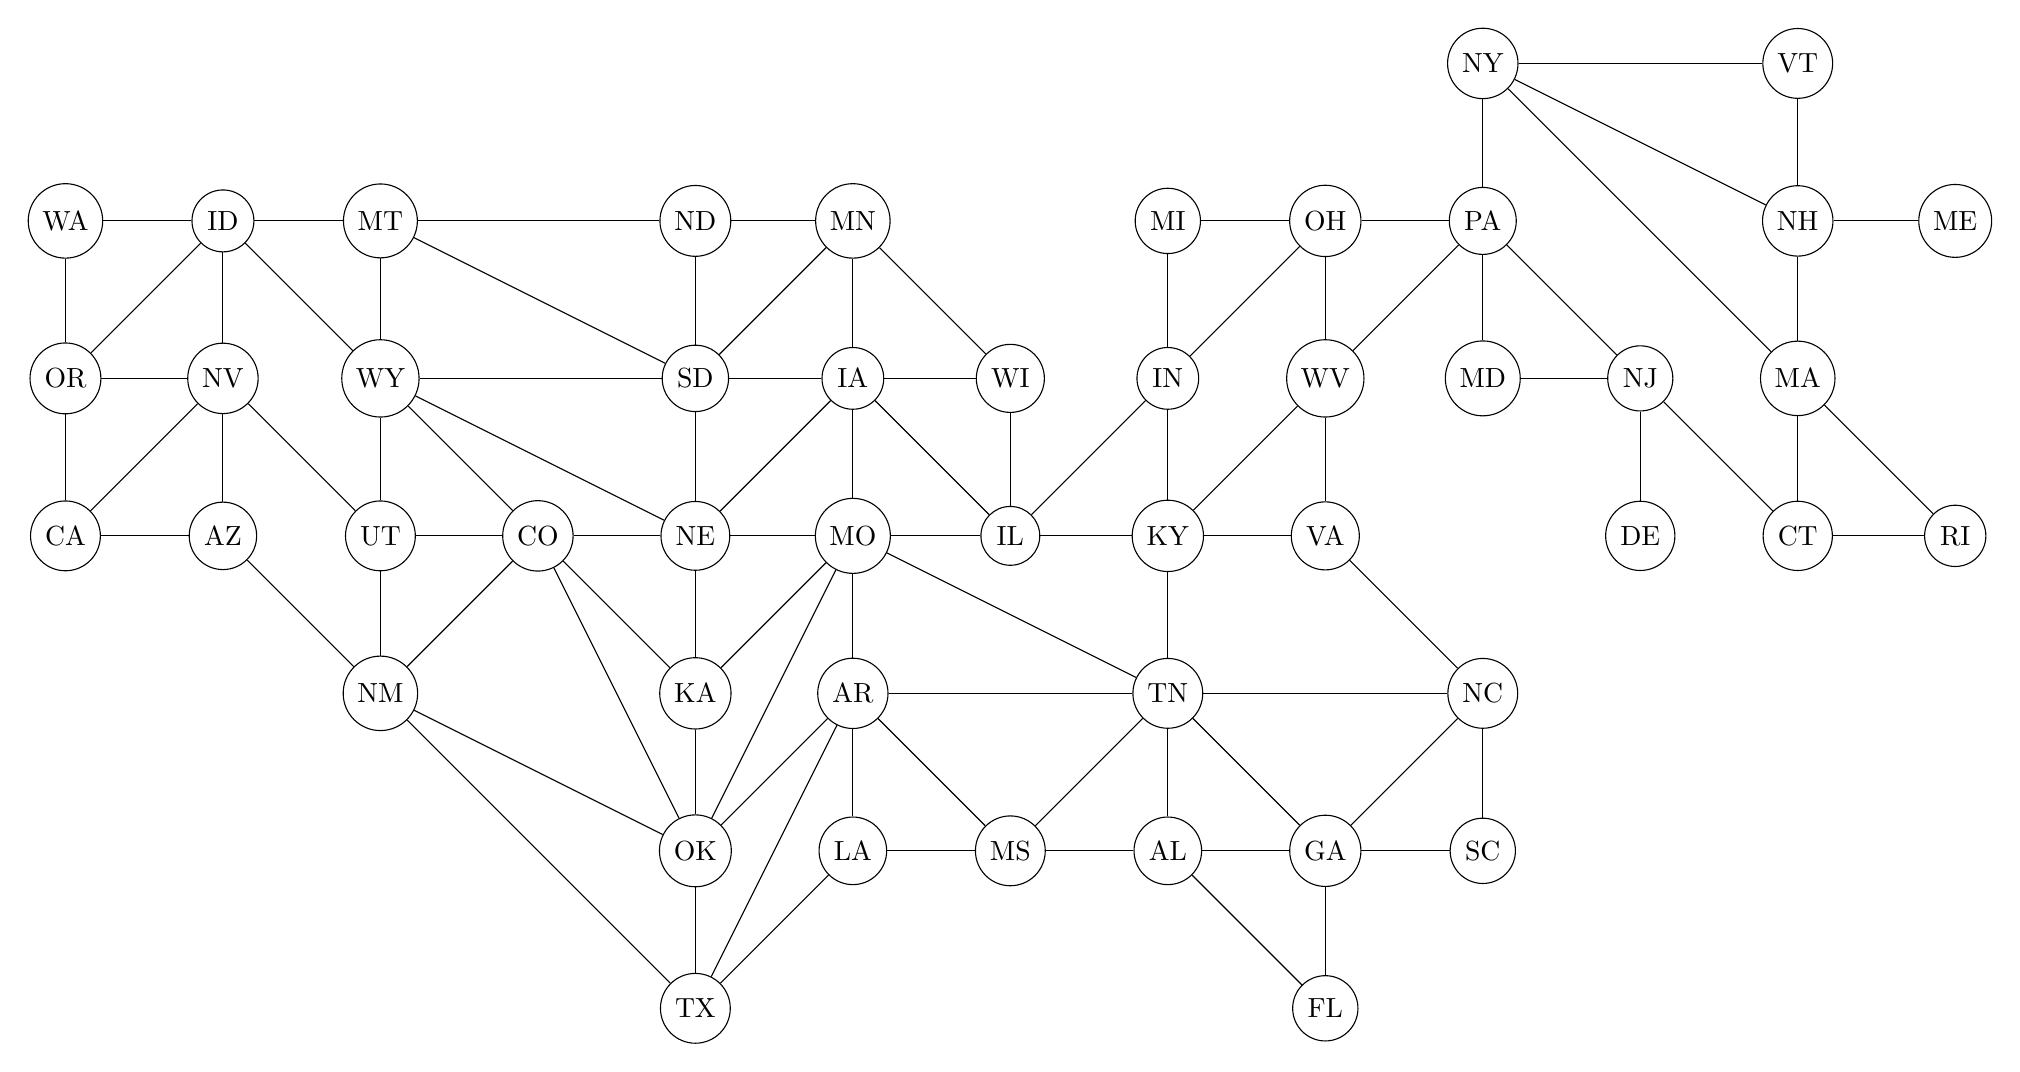
\begin{tikzpicture}
\node[circle,draw] (WA) at (0,10){WA};
\node[circle,draw] (OR) at (0,8){OR};
\node[circle,draw] (CA) at (0,6){CA};
\node[circle,draw] (ID) at (2,10){ID};
\node[circle,draw] (NV) at (2,8){NV};
\node[circle,draw] (AZ) at (2,6){AZ};
\node[circle,draw] (MT) at (4,10){MT};
\node[circle,draw] (WY) at (4,8){WY};
\node[circle,draw] (UT) at (4,6){UT};
\node[circle,draw] (NM) at (4,4){NM};
\node[circle,draw] (CO) at (6,6){CO};
\node[circle,draw] (ND) at (8,10){ND};
\node[circle,draw] (SD) at (8,8){SD};
\node[circle,draw] (NE) at (8,6){NE};
\node[circle,draw] (KA) at (8,4){KA};
\node[circle,draw] (OK) at (8,2) {OK};
\node[circle,draw] (TX) at (8,0){TX};
\node[circle,draw] (MN) at (10,10){MN};
\node[circle,draw] (IA) at (10,8){IA};
\node[circle,draw] (MO) at (10,6){MO};
\node[circle,draw] (AR) at (10,4){AR};
\node[circle,draw] (LA) at (10,2){LA};
\node[circle,draw] (WI) at (12,8){WI};
\node[circle,draw] (IL) at (12,6){IL};
\node[circle,draw] (MS) at (12,2){MS};
\node[circle,draw] (MI) at (14,10){MI};
\node[circle,draw] (IN) at (14,8){IN};
\node[circle,draw] (KY) at (14,6){KY};
\node[circle,draw] (TN) at (14,4){TN};
\node[circle,draw] (AL) at (14,2){AL};
\node[circle,draw] (OH) at (16,10){OH};
\node[circle,draw] (WV) at (16,8){WV};
\node[circle,draw] (VA) at (16,6){VA};
\node[circle,draw] (GA) at (16,2){GA};
\node[circle,draw] (FL) at (16,0){FL};
\node[circle,draw] (NY) at (18,12){NY};
\node[circle,draw] (PA) at (18,10){PA};
\node[circle,draw] (MD) at (18,8){MD};
\node[circle,draw] (NC) at (18,4){NC};
\node[circle,draw] (SC) at (18,2){SC};
\node[circle,draw] (NJ) at (20,8){NJ};
\node[circle,draw] (DE) at (20,6){DE};
\node[circle,draw] (VT) at (22,12){VT};
\node[circle,draw] (NH) at (22,10){NH};
\node[circle,draw] (MA) at (22,8){MA};
\node[circle,draw] (CT) at (22,6){CT};
\node[circle,draw] (RI) at (24,6){RI};
\node[circle,draw] (ME) at (24,10){ME};

	
\foreach \from/\to in {CA/OR,OR/WA,WA/ID,ID/OR,ID/NV,OR/NV,NV/AZ,CA/AZ,CA/NV,ID/MT,MT/ND,MT/SD,ID/WY,MT/WY,WY/UT,WY/CO,WY/NE,WY/SD,NV/UT,NM/AZ,NM/UT,TX/OK,NM/CO,NM/TX,NM/OK,CO/NE,CO/KA,CO/OK,CO/UT,ND/SD,SD/NE,NE/KA,KA/OK,MN/ND,MN/SD,MN/IA,IA/SD,IA/NE,IA/MO,MO/NE,MO/KA,MO/OK,MO/AR,MO/TN,AR/OK,AR/TX,AR/LA,LA/TX,MN/WI,IA/WI,WI/IL,IL/IA,IL/MO,IL/KY,MS/AR,MS/LA,MI/IN,MI/OH,IN/IL,IN/KY,KY/TN,TN/MS,TN/AR,TN/AL,AL/MS,AL/FL,OH/IN,OH/WV,WV/VA,WV/KY,WV/VA,VA/KY,VA/NC,NC/GA,NC/TN,NC/SC,SC/GA,GA/AL,GA/TN,GA/FL,PA/OH,PA/WV,PA/NJ,PA/MD,MD/NJ,NJ/DE,NJ/CT,CT/RI,NY/PA,NY/VT,NY/NH,NY/MA,VT/NH,NH/MA,MA/CT,MA/RI,NH/ME}
\draw (\from) -- (\to);
\end{tikzpicture}
\]
	
	
\end{document}
